\documentclass[a4paper, 12pt]{article}
%\usepackage{enumerate}
\usepackage[utf8]{vietnam}
\usepackage[utf8]{inputenc}
\usepackage[english]{babel}
\usepackage{graphicx}
\usepackage{hyperref}
\hypersetup{
    colorlinks=true,
    linkcolor=blue,
    filecolor=magenta,      
    urlcolor=cyan,
}

\title{CTT451 - Proposed Method\\ Single hand gesture recognition}
\date{\today}

\begin{document}

\begin{center} 
\large VNUHCM - University of Science\\
Faculty of Information Technology\\
Advanced Program in Computer Science
\end{center}

\begingroup
\let\newpage\relax
\maketitle
\endgroup

\textbf{Group members:}
\begin{enumerate}
	\item Student 1453034: Huỳnh Thiên Phước
	\item Student 1453058: Trần Sơn Vũ
\end{enumerate}

\section{Introduction}
Single hand gesture recognition can be defined as the process of analyzing and understanding meaningful movements of the hand. It acquires paramount importance due to its applications in sign language recognition, which provides better communication between deaf and dumb people and normal people. In addition, it can also be used to make wired gloves, depth-aware cameras, stereo cameras and gesture-based controllers.
\section{Project Details}

\subsection{Theory}
We will use the Kalman filter, k-means clustering, hand extraction, HoG feature extraction and SVM classification

\subsection{Methodology}
Firstly, we will use the Kalman filter to output a bounding box surrounding the hand by tracking the hand motion. Then we isolate the target by perform a k-mean clustering step based on the Lab colorspace. Next, we will perform hand extraction and then extract HoG features. Finally, we will train and test a SVM classifier using the extracted features.
\begin{figure}[!ht]
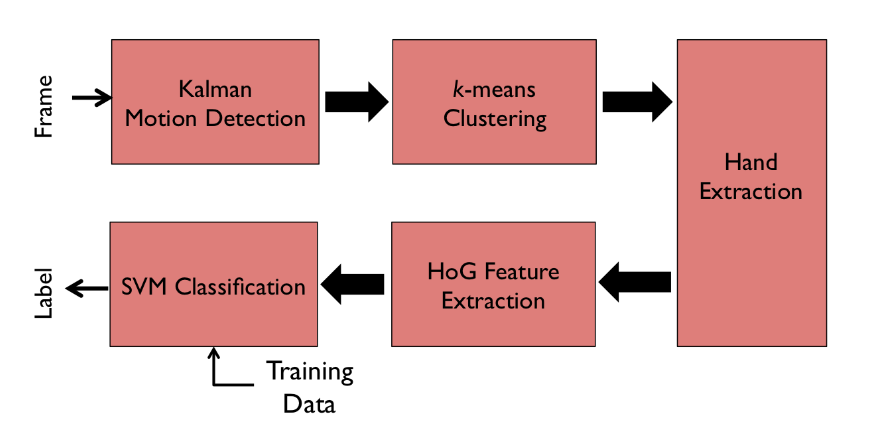
\includegraphics[width=\textwidth]{overview.png}
\caption{Overview of the proposed gesture recognition system}
\label{fig:foo}
\end{figure}

%\subsubsection*{Policy applications: \ldots}
\subsection{Time plan for project}
20/11 - 26/11 Find out about the Kalman filter, k-mean clustering and some hand extraction and code them. \newline
27/11 - 03/12 Find out about HoG feature extraction, SVM classification and code them. \newline
04/12 - 10/12 Merge them. \newline
11/12 - 17/12 Train and test \newline

\bibliographystyle{unsrt}
\begin{thebibliography}{1}
\bibitem{latexcompanion} 
Christos G. Bampis and Jinseok Choi
\textit{\href{http://christosbampis.info/wp-content/uploads/2015/05/DigVidProject_2015.pdf}{Single-hand gesture recognition using image/video processing and machine learning techniques}}.
\end{thebibliography}

\end{document}